\section{ПОРОЖДАЮЩИЕ ПАТТЕРНЫ}

Порождающие паттерны проектирования абстрагируют процесс инстанцирования.
Они помогут сделать систему независимой от способа создания, композиции
и представления объектов. Паттерн, порождающий классы, использует наследование,
чтобы варьировать инстанцируемый класс, а паттерн, порождающий объекты,
делегирует инстанцирование другому объекту.

Для порождающих паттернов актуальны две темы. Во-первых, эти паттерны
инкапсулируют знания о конкретных классах, которые применяются в системе.
Во-вторых, они скрывают детали того, как эти классы создаются и стыкуются.
Единственная информация об объектах, известная системе, --- это их интерфейсы,
определенные с помощью абстрактных классов.
Следовательно, порождающие паттерны обеспечивают большую гибкость при решении
вопроса о том, что создается, кто это создает, как и когда.
Можно собрать систему из «готовых» объектов с самой различной структурой и
функциональностью статически (на этапе компиляции) или динамически (во время выполнения).

Есть два наиболее распространенных способа параметризовать систему классами
создаваемых ей объектов. Первый способ --- порождение подклассов от класса,
создающего объекты. Он соответствует паттерну фабричный метод. Основной
недостаток метода: требуется создавать новый подкласс лишь для того, чтобы
изменить класс продукта. И таких изменений может быть очень много. Например,
если создатель продукта сам создается фабричным методом, то придется
замещать и создателя тоже.

Другой способ параметризации системы в большей степени основан на композиции
объектов. Вы определяете объект, которому известно о классах объектов-продуктов,
и делаете его параметром системы. Это ключевой аспект таких
паттернов, как абстрактная фабрика, строитель и прототип. Для всех трех
характерно создание «фабричного объекта», который изготавливает продукты.
В абстрактной фабрике фабричный объект производит объекты разных классов.
Фабричный объект строителя постепенно создает сложный продукт, следуя
специальному протоколу. Фабричный объект прототипа изготавливает продукт путем
копирования объекта-прототипа. В последнем случае фабричный объект
и прототип --- это одно и то же, поскольку именно прототип отвечает за возврат
продукта.

Иногда допустимо выбирать между тем или иным порождающим паттерном.
Например, есть случаи, когда с пользой для дела можно использовать как прототип,
так и абстрактную фабрику. В других ситуациях порождающие паттерны
дополняют друг друга. Так, применяя строитель, можно использовать другие паттерны
для решения вопроса о том, какие компоненты нужно строить, а прототип
часто реализуется вместе с одиночкой.

\section{ПОРОЖДАЮЩИЙ ПАТТЕРН <<СТРОИТЕЛЬ>>}

Паттерн <<строитель>> отделяет конструирование сложного объекта от его представления,
так что в результате одного и того же процесса конструирования могут получаться
различные представления.

\subsection{Применимость}

Паттерн <<строитель>> в следующих случаях:
\begin{itemize}
\item
  алгоритм создания сложного объекта не должен зависеть от того, из каких
  частей состоит объект и как они стыкуются между собой;
\item
  процесс конструирования должен обеспечивать различные представления
  конструируемого объекта.
\end{itemize}

\subsection{Структура паттерна}

Диаграмма классов паттерна <<строитель>> приведена на рисунке~\ref{fig:builder_uml}.

\begin{figure}[h!]
  \centering
  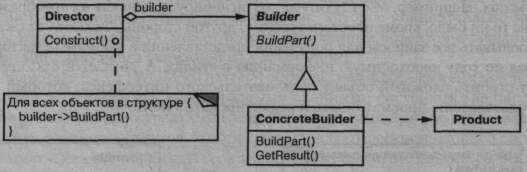
\includegraphics[width=150mm]{pic/builder_uml.png}
  \caption{Диаграмма классов паттерна <<строитель>>}
  \label{fig:builder_uml}
\end{figure}

Перечислим классы, участвующие в паттерне <<строитель>>.

\textbf{Builder} --- строитель: задает абстрактный интерфейс
для создания частей объекта Product.

\textbf{ConcreteBuilder} --- конкретный строитель: 
\begin{itemize}
\item
  конструирует и собирает вместе части продукта посредством реализации
  интерфейса Builder;
\item
  определяет создаваемое представление и следит за ним;
\item
  предоставляет интерфейс для доступа к продукту.
\end{itemize}

\textbf{Director} --- распорядитель: конструирует объект, пользуясь интерфейсом Builder.

\textbf{Product} --- продукт:
\begin{itemize}
\item
  представляет сложный конструируемый объект.
  ConcreteBuilder строит внутреннее представление продукта
  и определяет процесс его сборки;
\item
  включает классы, которые определяют составные части,
  в том числе интерфейсы для сборки конечного результата из частей.
\end{itemize}

\subsection{Отношения между участниками паттерна}
На рисунке~\ref{fig:builder_uml_2} изображены взаимоотношения
строителя и распорядителя с клиентом.

\begin{figure}[h!]
  \centering
  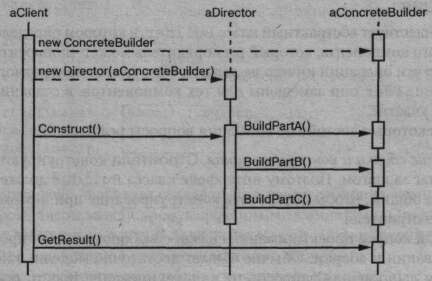
\includegraphics[width=150mm]{pic/builder_uml_2.png}
  \caption{Диаграмма взаимодействия паттерна <<строитель>>}
  \label{fig:builder_uml_2}
\end{figure}

\begin{itemize}
\item
клиент создает объект-распорядитель Director и конфигурирует его
нужным объектом-строителем Builder;
\item
  распорядитель уведомляет строителя о том, что нужно построить 
  очередную часть продукта;
\item
  строитель обрабатывает запросы распорядителя и добавляет новые
  части к продукту;
\item
  клиент забирает продукт у строителя.
\end{itemize}

\subsection{Результаты использования паттерна}

Плюсы и минусы паттерна строитель и его применения:
\begin{itemize}
\item
  Позволяет изменять внутреннее представление продукта.
  Объект Builder предоставляет распорядителю абстрактный интерфейс
  для конструирования продукта, за которым он может скрыть представление
  и внутреннююструктуру продукта, а также процесс его сборки.
  Поскольку продукт конструируется через абстрактный интерфейс,
  то для изменения внутреннего представления достаточно всего лишь
  определить новый вид строителя.
\item
  Изолирует код, реализующий конструирование и представление.
  Паттерн <<строитель>> улучшает модульность, инкапсулируя способ конструирования
  и представления сложного объекта. Клиентам ничего не надо знать о 
  классах, определяющих внутреннюю структуру продукта, они отсутствуют
  в интерфейсе строителя.
\item
  Каждый конкретный строитель ConcreteBuilder содержит весь код,
  необходимый для создания и сборки конкретного вида продукта. Код пишется
  только один раз, после чего разные распорядители могут использовать
  его повторно для построения вариантов продукта из одних и тех же частей.
\end{itemize}

\subsection{Пример использования}

Программа, в которую заложена возможность распознавания и чтения документа
в формате RTF (Rich Text Format), должна также «уметь» преобразовывать
его во многие другие форматы, например в простой ASCII-текст или в
представление, которое можно отобразить в виджете для ввода текста.
Однако число вероятных преобразований заранее неизвестно.
Поэтому должна быть обеспечена возможность без труда добавлять новый конвертор.

Таким образом, нужно сконфигурировать класс RTFReader с помощью объекта
Text Converter, который мог бы преобразовывать RTF в другой текстовый
формат. При разборе документа в формате RTF класс RTFReader вызывает
TextConverter для выполнения преобразования. Всякий раз, как RTFReader
распознает лексему RTF (простой текст или управляющее слово), для ее
преобразования объекту TextConverter посылается запрос.
Объекты TextConverter отвечают как за преобразование данных,
так и за представление лексемы в конкретном формате.

Подклассы TextConverter специализируются на различных преобразованиях
и форматах. Например, ASCIIConverter игнорирует запросы на преобразование
чего бы то ни было, кроме простого текста. С другой стороны, TeXConverter будет
реализовывать все запросы для получения представления в формате редактора TJX,
собирая по ходу необходимую информацию о стилях. A Text Widget Converter
станет строить сложный объект пользовательского интерфейса, который позволит
пользователю просматривать и редактировать текст.

Диаграмма классов для рассматриваемого функционала текстового
редактора представлена на рисунке~\ref{fig:rtf_uml}.

\begin{figure}[h!]
  \centering
  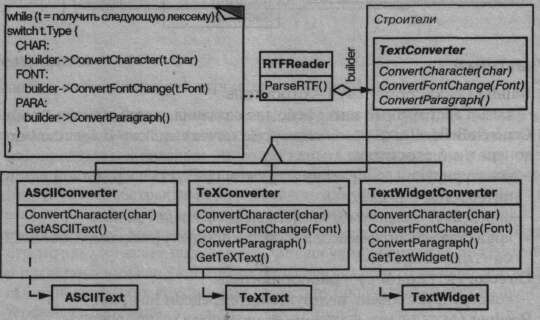
\includegraphics[height=87mm]{pic/rtf_uml.png}
  \caption{Диаграмма классов подсистемы текстового редактора}
  \label{fig:rtf_uml}
\end{figure}

Класс каждого конвертора принимает механизм создания и сборки сложного
объекта и скрывает его за абстрактным интерфейсом. Конвертор отделен от 
загрузчика, который отвечает за синтаксический разбор RTF-документа.

В паттерне строитель абстрагированы все эти отношения. В нем любой класс
конвертора называется строителем, а загрузчик --- распорядителем.
В применении к рассмотренному примеру строитель отделяет алгоритм интерпретации
формата текста (то есть анализатор RTF-документов) от того, как создается и
представляется документ в преобразованном формате. Это позволяет повторно использовать
алгоритм разбора, реализованный в RTFReader, для создания разных текстовых
представлений RTF-документов; достаточно передать в RTFReader различные подклассы 
класса Text Converter.

Материалы для ответа взяты из источника~\cite{gamma01}.